%==============================================================
%  ICON-LM: Fine-Tuning Language Models as Multi-Modal
%  Differential Equation Solvers --- Course Presentation
%
%  Compile with:  pdflatex Presentation.tex
%
%  Target: 7 minutes total, two presenters (about 3.5 min each).
%  Live flow: title + 7 content slides; conclusion/details are backup.
%==============================================================

\documentclass[10pt,aspectratio=169]{beamer}

%-------------------- THEME ----------------------------------
\usetheme{Madrid}
\usecolortheme{seahorse}
\useinnertheme{rectangles}
\useoutertheme{infolines}

\definecolor{iconblue}{RGB}{30,72,116}
\definecolor{iconaccent}{RGB}{198,108,42}
\definecolor{iconlight}{RGB}{235,240,247}
\setbeamercolor{structure}{fg=iconblue}
\setbeamercolor{frametitle}{bg=iconblue,fg=white}
\setbeamercolor{title}{bg=iconblue,fg=white}
\setbeamercolor{block title}{bg=iconblue,fg=white}
\setbeamercolor{block body}{bg=iconlight,fg=black}

%-------------------- PACKAGES -------------------------------
\usepackage[utf8]{inputenc}
\usepackage{amsmath,amssymb,amsthm}
\usepackage{bm}
\usepackage{booktabs}
\usepackage{array}
\usepackage{graphicx}
\usepackage{tikz}
\usepackage{pgfplots}
\pgfplotsset{compat=1.17}
\usetikzlibrary{positioning,arrows.meta,calc,fit,backgrounds,shapes.geometric}

\setbeamertemplate{itemize items}[circle]
\setlength{\leftmargini}{1.4em}

% math shortcuts
\newcommand{\bool}{\operatorname{bool}}

%-------------------- METADATA -------------------------------
\title[ICON-LM]{Fine-Tuning Language Models as\\Multimodal Differential Equation Solvers}
\subtitle{ICON-LM \,---\, Yang, Liu, \& Osher (2024)}
\author[]{Aditya Patil \and Dhruv Patel}
\institute[MATH 270A]{MATH 270A Final Project}
\date{June 3, 2026}

\IfFileExists{toy_multiphysics/metrics.tex}{\input{toy_multiphysics/metrics.tex}}{}
\IfFileExists{toy_multiphysics/eval_metrics.tex}{\input{toy_multiphysics/eval_metrics.tex}}{}
\providecommand{\ToyGrid}{$64\times 64$}
\providecommand{\ToyFrames}{4}
\providecommand{\ToyShots}{4}
\providecommand{\ToyTrainDevice}{CUDA/MPS}
\providecommand{\ToyTrainTime}{run on sci06}
\providecommand{\ToyTestRel}{from \texttt{train.log}}
\providecommand{\ToyContextSummary}{run \texttt{evaluate.py}}
\providecommand{\ToyInverseAcc}{run \texttt{evaluate.py}}

%==============================================================
\begin{document}
%==============================================================

%----- Slide 1: Title ----------------------------------------
\begin{frame}
  \titlepage
\end{frame}

%==============================================================
% ============== PRESENTER 1 (slides 2--5) ====================
%==============================================================

\section{Motivation and the ICON-LM idea}

%----- Slide 2: Motivation + proposal ------------------------
\begin{frame}{Why ICON-LM?}
  \begin{columns}[T,onlytextwidth]
    \column{0.50\textwidth}
      \textbf{Classic Operator Learning}
      \begin{itemize}\setlength\itemsep{0.16em}
        \item Trains 1 neural operator for 1 map \\ $T:c\mapsto u$
        \item Change the PDE, coefficients, or task \\
        $\Rightarrow$ Retrain or fine-tune
        \item Hard to inject equation knowledge without redesigning the model
      \end{itemize}
      \vspace{0.45em}
      \textbf{ICON-LM}
      \begin{itemize}\setlength\itemsep{0.16em}
        \item Treat examples $\{(c_j,u_j)\}$ as the \emph{context}
        \item Treat a text/equation caption $\kappa$ as another input modality
        \item Predict the query function in one forward pass with no weight updates
      \end{itemize}
    \column{0.48\textwidth}
      \begin{block}{Changes introduced by ICON-LM}
        \begin{enumerate}\setlength\itemsep{0.16em}
          \item \textbf{Multimodal prompts}: Data examples with a caption to describe the operator
          \item \textbf{LM-style training}: 1 transformer encoder trained by next-\emph{function} prediction
        \end{enumerate}
      \end{block}
      \vspace{0.2em}
      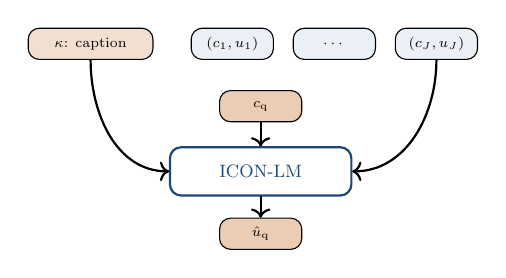
\begin{tikzpicture}[scale=0.72,transform shape]
        \tikzset{
          tok/.style={draw,rounded corners,minimum width=1.45cm,minimum height=0.55cm,fill=iconlight,font=\scriptsize},
          captok/.style={tok,fill=iconaccent!22,minimum width=2.2cm},
          qtok/.style={tok,fill=iconaccent!35}
        }
        \node[captok] (cap) at (0,0) {$\kappa$: caption};
        \node[tok] (e1) at (2.5,0) {$(c_1,u_1)$};
        \node[tok] (e2) at (4.3,0) {$\cdots$};
        \node[tok] (eJ) at (6.1,0) {$(c_J,u_J)$};
        \node[qtok] (cq) at (3.0,-1.1) {$c_{\text{q}}$};
        \node[draw,thick,iconblue,rounded corners,minimum width=3.2cm,minimum height=0.85cm] (T) at (3.0,-2.25) {\small ICON-LM};
        \node[qtok] (uhat) at (3.0,-3.35) {$\hat{u}_{\text{q}}$};
        \draw[->,thick] (cap.south) to[out=270,in=180] (T.west);
        \draw[->,thick] (eJ.south) to[out=270,in=0] (T.east);
        \draw[->,thick] (cq) -- (T);
        \draw[->,thick] (T) -- (uhat);
      \end{tikzpicture}
      \vspace{0.2em}

      {\scriptsize Paper benchmark: 19 ODE/PDE/control operator families.}
  \end{columns}
\end{frame}

\section{Architecture}

%----- Slide 3: Architecture overview ------------------------
\begin{frame}{Architecture}
  \begin{columns}[onlytextwidth]
    \column{0.50\textwidth}
      \textbf{From encoder--decoder ICON to ICON-LM}
      \begin{itemize}\setlength\itemsep{0.1em}
        \item Original ICON: two transformers ($\sim 31.6$M params).
        \item ICON-LM: a single GPT-style encoder ($\approx 15.8$M).

      \end{itemize}
      \vspace{0.4em}
      \textbf{Tokens}:
      \begin{itemize}\setlength\itemsep{0.1em}
        \item Three token types per example: \textbf{C}ondition, \textbf{U} (QoI), \textbf{Q}uery.
        \item Query tokens carry spatial \emph{locations}; values zeroed out (model fills these in).
      \end{itemize}
    \column{0.48\textwidth}
      \vspace*{\fill}
      \centering
      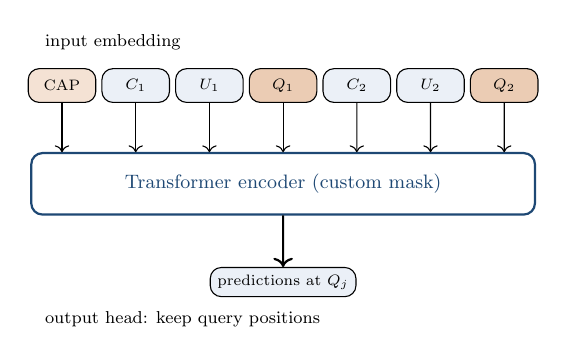
\begin{tikzpicture}[scale=0.78,transform shape]
        \tikzset{tok/.style={draw,rounded corners,minimum width=1.1cm,minimum height=0.55cm,font=\scriptsize}}
        \node[tok,fill=iconaccent!20] (cap)  at (0,0)   {CAP};
        \node[tok,fill=iconlight]      (c1) at (1.2,0) {$C_1$};
        \node[tok,fill=iconlight]      (q1) at (2.4,0) {$U_1$};
        \node[tok,fill=iconaccent!35]  (qq1) at (3.6,0) {$Q_1$};
        \node[tok,fill=iconlight]      (c2) at (4.8,0) {$C_2$};
        \node[tok,fill=iconlight]      (q2) at (6.0,0) {$U_2$};
        \node[tok,fill=iconaccent!35]  (qq2) at (7.2,0) {$Q_2$};
        \node[draw,thick,iconblue,fill=white,rounded corners,
              minimum width=8.2cm,minimum height=1cm] (tr) at (3.6,-1.6) {\small Transformer encoder (custom mask)};
        \node[draw,rounded corners,minimum width=1.6cm,fill=iconlight,font=\scriptsize] (h1) at (3.6,-3.2) {predictions at $Q_j$};
        \foreach \n in {cap,c1,q1,qq1,c2,q2,qq2}{\draw[->] (\n) -- (tr.north -| \n);}
        \draw[->,thick] (tr) -- (h1);
        \node[font=\footnotesize,anchor=west] at (-0.4,0.7) {input embedding};
        \node[font=\footnotesize,anchor=west] at (-0.4,-3.8) {output head: keep query positions};
      \end{tikzpicture}
      \vspace*{\fill}
  \end{columns}
\end{frame}

\section{The Attention Mask}

%----- Slide 4: Custom mask (centerpiece) --------------------
\begin{frame}{The Custom Mask: Preventing Leakage}
  \begin{columns}[T,onlytextwidth]
    \column{0.48\textwidth}
      \textbf{Why it is needed}
      \begin{itemize}\setlength\itemsep{0.2em}
        \item Each example has an input function $C_j$ and output function $U_j$
        \item To predict $U_j$, the query tokens $Q_j$ may use previous example pairs alongside $C_j$
        \item But $Q_j$ must not attend to the current output $U_j$, because that is the answer
        \item Previous queries unused as context
      \end{itemize}

      \vspace{0.35em}
      \textbf{Key idea}
      \begin{itemize}\setlength\itemsep{0.2em}
        \item White blocks are allowed context, grey blocks are blocked to prevent answer leakage.
      \end{itemize}
      \[
        Q_j \text{ can see } (C_1,U_1),\dots,(C_{j-1},U_{j-1}),C_j
      \]
      \[
        Q_j \text{ cannot see } U_j
      \]

    \column{0.50\textwidth}
      \begin{center}
        \includegraphics[
          width=\linewidth,
          height=5.45cm,
          keepaspectratio
        ]{mask.png}

        \vspace{0.15em}
        {\scriptsize Figure 3 from Yang, Liu, \& Osher}
      \end{center}
  \end{columns}
\end{frame}


%----- Slide 5: Training -------------------------------------
\begin{frame}{Training}
  \begin{block}{Autoregressive loss across examples}
    For each $J = 0,1,\dots,I-1$ in an $I$-example prompt, predict $u_{J+1}$ from earlier examples and the caption:
    \[
      \hat{u}_{J+1} \;=\; T_\theta\!\left[c_{J+1};\,\{(c_i,u_i)\}_{i=1}^{J},\,\kappa\right].
    \]
    \[
      \mathcal{L}_{\text{prompt}} \;=\; \sum_{J=0}^{I-1}\bigl\lVert\hat{u}_{J+1}-u_{J+1}\bigr\rVert^2.
    \]
  \end{block}
\begin{itemize}\setlength\itemsep{0.1em}
    \item One prompt simultaneously trains \emph{every} few-shot count $J$.
    \item With a caption, $J=0$ contributes (zero-shot); without, training starts at $J=1$.
    \item Multi-modal loss $=$ loss with caption $+$ loss without caption.
    \item \textbf{Inference}: append a input condition $c_{\text{q}}$ + query tokens, one forward pass.
  \end{itemize}
\end{frame}

%==============================================================
% ============== PRESENTER 2 (slides 6--8) ====================
%==============================================================

\section{Results}

%----- Slide 6: Paper results --------------------------------
\begin{frame}{Paper Results}
  \begin{columns}[T,onlytextwidth]
    \column{0.45\textwidth}
      \begin{block}{Main empirical claims}
        \begin{itemize}\setlength\itemsep{0.18em}
          \item \textbf{Smaller and stronger}: ICON-LM improves on encoder--decoder ICON with roughly half the parameters
          \item \textbf{Captions matter}: Precise captions enable zero-shot prediction; vague captions reduce the number of examples needed
        \end{itemize}
      \end{block}
      \vspace{0.25em}
      \begin{center}
        \scriptsize
        \begin{tabular}{lcc}
          \toprule
          \textbf{Model} & \textbf{Params} & \textbf{Use at test time}\\
          \midrule
          Encoder--decoder ICON & $\sim 31.6$M & examples only\\
          ICON-LM & $\sim 15.8$M & examples + caption\\
          \bottomrule
        \end{tabular}
      \end{center}
    \column{0.53\textwidth}
      \begin{center}
        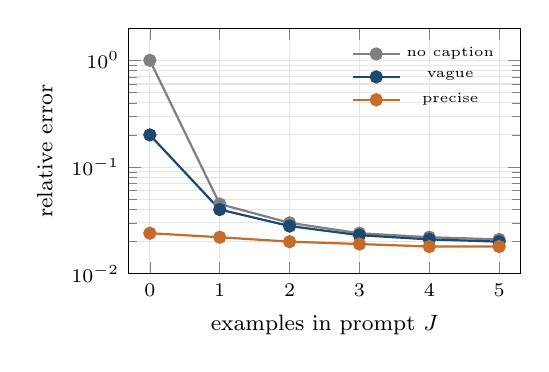
\begin{tikzpicture}
          \begin{semilogyaxis}[
            width=6.55cm,height=4.7cm,
            xlabel={\footnotesize examples in prompt $J$},
            ylabel={\footnotesize relative error},
            xmin=-0.3,xmax=5.3,ymin=0.01,ymax=2,
            xtick={0,1,2,3,4,5},
            tick label style={font=\scriptsize},
            legend style={font=\tiny,at={(0.97,0.97)},anchor=north east,draw=none,fill=none},
            grid=both,grid style={gray!20}
          ]
            \addplot[color=gray,thick,mark=*]       coordinates {(0,1.0)(1,0.045)(2,0.030)(3,0.024)(4,0.022)(5,0.021)};
            \addplot[color=iconblue,thick,mark=*]   coordinates {(0,0.20)(1,0.040)(2,0.028)(3,0.023)(4,0.021)(5,0.020)};
            \addplot[color=iconaccent,thick,mark=*] coordinates {(0,0.024)(1,0.022)(2,0.020)(3,0.019)(4,0.018)(5,0.018)};
            \legend{no caption, vague, precise}
          \end{semilogyaxis}
        \end{tikzpicture}
      \end{center}
      \vspace{-0.35em}
      {\scriptsize Caption benefit is most visible at $J=0$ or $J=1$, exactly where numerical examples are sparse.}
  \end{columns}
\end{frame}

\section{Discussion}

%----- Slide 7: Ablation -------------------------------------
\begin{frame}{Ablation}
  \begin{block}{Zero-shot relative error with precise captions}
    \centering
    \begin{tabular}{lccc}
      \toprule
      \textbf{GPT-2 init.} & \textbf{Train} & \textbf{Test} & \textbf{Gap} \\
      \midrule
      Pre-trained weights         & 2.30\,\% & 2.44\,\% & \textbf{0.14\,\%} \\
      Random weights & 2.07\,\% & 3.08\,\% & 1.01\,\% \\
      \bottomrule
    \end{tabular}
  \end{block}
  \begin{itemize}\setlength\itemsep{0.2em}
    \item \textbf{Pre-trained} GPT-2 generalizes better across captions \begin{itemize}
        \item Suggests language priors transfer
    \end{itemize}
    \item \textbf{Random init} can win in few-shot settings 
    \begin{itemize}
        \item Suggests language pre-training is not always ideal for numerical prediction
    \end{itemize}
  \end{itemize}
\end{frame}

\section{Our experiment}

%----- Slide 8: Our reproduction placeholder -----------------
\begin{frame}{Reproduction on Burgers' Equation}
  \small
  \begin{columns}[T,onlytextwidth]
    \column{0.47\textwidth}
      \textbf{What we reproduced}
      \vspace{0.2em}
      \begin{block}{}
        \centering
        $\displaystyle u_t + u\,u_x \;=\; \nu\,u_{xx}$
      \end{block}
      \vspace{0.1em}
      \begin{itemize}\setlength\itemsep{0.10em}
        \item Reproduced ICON-LM architecture: custom mask + next-function loss
        \item  Applied to 1D viscous Burgers' equation, operator family indexed by $\nu$.
        \item 2.2M-parameter transformer; 5{,}000 gradient steps.
        \item Optional captions via frozen MiniLM embeddings.
      \end{itemize}
    \column{0.50\textwidth}
      \begin{center}
  \IfFileExists{panel_a.png}{%
    \includegraphics[width=\linewidth,height=4.65cm,keepaspectratio]{panel_a.png}%
  }{%
    \fbox{\parbox[c][3.65cm][c]{0.92\linewidth}{\centering
      \small Few-shot context-scaling panel missing.\\[0.45em]
      \scriptsize Generate \texttt{panel\_a.png}.
    }}%
  }
\end{center}
  \end{columns}
\end{frame}

%==============================================================
% ============ BACKUP SLIDES (not in 7-min flow) ==============
%==============================================================

\appendix

\section{Backup}

\begin{frame}{Conclusion}
  \begin{block}{Key Takeaway}
    ICON-LM turns operator learning into a language-model-style problem:
    examples are context, functions are tokens, captions are side information,
    and a custom mask makes next-function prediction possible without leakage.
  \end{block}
  \vspace{0.25em}
  \begin{columns}[T,onlytextwidth]
    \column{0.50\textwidth}
      \textbf{Why it works}
      \begin{itemize}\setlength\itemsep{0.18em}
        \item Single transformer encoder.
        \item One training sequence supervises all few-shot levels at once.
        \item Captions help when examples are scarce.
      \end{itemize}
    \column{0.48\textwidth}
      \vspace{2em}
      \begin{center}
        \large\textit{Thanks for listening!}
      \end{center}
  \end{columns}
\end{frame}

\begin{frame}{References}
  \footnotesize
  \begin{itemize}\setlength\itemsep{0.15em}
    \item L. Yang, S. Liu, S. J. Osher. \textit{Fine-Tune Language Models as Multi-Modal Differential Equation Solvers}, 2024. (\textbf{The paper.})
    \item L. Yang, S. Liu, T. Meng, S. J. Osher. \textit{In-context operator learning with data prompts for differential equation problems}. PNAS 120 (2023).
    \item Z. Li, N. Kovachki, K. Azizzadenesheli, et al. \textit{Fourier Neural Operator for Parametric PDEs}, ICLR 2021.
    \item L. Lu, P. Jin, G. Pang, Z. Zhang, G. E. Karniadakis. \textit{Learning nonlinear operators via DeepONet}, Nature MI 2021.
    \item A. Radford, J. Wu, R. Child, et al. \textit{Language Models are Unsupervised Multitask Learners} (GPT-2), 2019.
    \item G. E. Karniadakis et al. \textit{Physics-informed machine learning}, Nature Reviews Physics 3 (2021).
    \item Code: \texttt{github.com/LiuYangMage/in-context-operator-networks}
  \end{itemize}
\end{frame}

\end{document}
